    \subsection{Вырезание}

    Рассмотрим тройку $B \subset A \subset X$. Тогда вложение индуцирует отображение
    \[ H_{k}(X - B, A - B) \to H_{k}(X, A). \]

    Вообще говоря, вырезание даёт хорошую технику вычисления относительных гомологий:

    \begin{theorem}[О вырезании]\label{CuttingTheorem}
        Пусть даны пространства $Z \subset A \subset X$, причем $\Cl(Z) \subset \Int(A)$. Тогда вложение
        $(X - Z, A - Z) \hookrightarrow (X, A)$ индуцирует изоморфизмы
        \[ H_{n}(X - Z, A - Z) \cong H_{n}(X, A) \]
        для всех $n$. Или, что эквивалентно: для подпространств $A, B \subset X$, внутренности которых покрывают $X$,
        включение $(B, A \cap B) \hookrightarrow (X, A)$  индуцирует изоморфизмы
        \[ H_{n}(B, A \cap B) \cong H_{n}(X, A) \quad \forall n. \]
    \end{theorem}

    \begin{proof}
        Докажем сначала эквивалентность формулировок.  Положим $B = X - Z, \ Z = X - B$.
        Тогда $A \cap B = A - Z$, а условие $\Cl(Z) \subset \Int(A)$ эквивалентно тому, что
        $X = \Int(A) \cup \Int(B)$, так как $X - \Int(B) = \Cl(Z)$. Теперь докажем вторую формулировку.

        Пусть $X = A \cup B$, обозначим соотвествующее покрытие $\cU = \{ A, B \}$. Для краткости будем обозначать группы
        $C^{\cU}_{n}(X)$, как $C_{n}(A + B)$\footnote{что на самом деле логично, так как цепи оттуда состоят из суммы цепей из $A$ и цепей из $B$}.

        Тогда, как мы помним из леммы об измельчении~\ref{IzmelchLemma} включение
        \[ C_{n}(A + B)/C_{n}(A) \hookrightarrow C_{n}(X)/C_{n}(A) \]
        индуцирует изоморфизм групп гомологий $H_{n}(A + B, A) \cong H_{n}(X, A)$.

        Теперь рассмотрим включение
        \[ C_{n}(B)/C_{n}(A \cap B) \hookrightarrow C_{n}(A + B, A). \]
        Оно очевидно индуцирует изоморфизм гомологий, так как обе факторгруппы свободные, а их базис~--- $n$-мерные сингулярные симплексы в $B$, не лежащие в $A$.
        Значит, мы получили требуемый изоморфизм
        \[ H_{n}(B, A \cap B) \cong H_{n}(A + B, A) \cong H_{n}(X, A). \]

    \end{proof}

    \subsection{Точная последовательность Майера-Вьеториса}

    Кроме длинной точной последовательности пары (теорема~\ref{LongExactSequenceOfPair}) для вычисления гомологий пары $(X, A)$
    есть и другая мощная техника для вычисления гомологий пространства $X$, тоже представляющая собой длинную точную последовательность.

    \begin{theorem}[Точная последовательность Майера-Вьеториса, простая версия]\label{Mayer–Vietoris_sequence}
        Пусть $X = A \cup B,$ где $A, B$~--- открытые и $A \cap B  = C \neq \varnothing$.
    Тогда имеет место следующая точная последовательность:
    \[ \ldots  H_{q}(A \cap B) \to H_{q}(A) \oplus H_{q}(B) \to H_{q}(X) \to H_{q - 1}(A \cap B) \to H_{q - 1}(A) \oplus H_{q - 1}(B)  \to \ldots \]
    \end{theorem}
    \begin{proof}
        Рассмотрим короткую точную последовательность  комплексов:
        \[ 0 \to C_{\bullet}(A \cap B) \xrightarrow[\varphi]{c \to (c, -c)} C_{\bullet}(A) \oplus C_{\bullet}(B) \xrightarrow[\psi]{(a, b) \to a + b} C_{\bullet}(A + B) \to 0\]
        Во-первых, заметим, что $\Ker{\varphi} = 0$, так как цепь  в $A \cap B$, которая является нулевой в $A$ (или в $B$) должна быть нулевой цепью.
        Во-вторых, очевидно, что $\psi\varphi = 0 \Rightarrow \Im{\varphi} \subset \Ker{\psi}$. Заметим, что для $(x, y) \in C_{n}(A) \oplus C_{n}(B)$
        имеем $x + y = 0 \Rightarrow y = -x$, а значит $x \in C_{n}(A \cap B)$ и $(x, y) \in \Im{\varphi}$. Это означает, что
        $\Ker{\psi} \subset \Im{\varphi}$. Точность в последнем члене следует просто из определения $C_{n}(A + B)$.

        Тогда эта короткая точная последовательность комплексов даёт нам точную последовательность гомологий. Остается лишь заметить, что
        также, как и в теореме о вырезании, $H_{\bullet}(A + B) = H_{\bullet}(A \cup B)$.
    \end{proof}

    \begin{remark}
       Эта не самая хорошая версия точной последовательности Майера-Вьеториса, так как условие на открытое покрытие серьезно мешает.
    \end{remark}   

    \subsection{Гомологии сфер}

    \begin{theorem}\label{SphereHomology}
        Для $n \neq 0$ гомологии сферы устроены следующим образом:
        \[ H_{i}(S^n) \cong \begin{cases} \Z, \quad i = n  \text{ или } i = n,\\ 0, \quad \text{иначе.}\end{cases} \]
        Или, иными словами,
        \[ \widetilde{H}_{i}(S^n) \cong \begin{cases} \Z, \quad i = n \\ 0, \quad \text{иначе.}\end{cases}\]
    \end{theorem}
    \begin{proof}
        Рассмотрим пару $(X, A) = (D^n, S^{n - 1})$, тогда $X/A \cong S^n$. Запишем для этой пары точную послеоватнльность приведенных гомологий:
        \[ \ldots \to \widetilde{H}_{q}\lr*{D^n} \to \widetilde{H}_{q}\lr*{D^n, S^{n - 1}} \to \widetilde{H}_{q - 1}\lr*{S^{n - 1}} \to \widetilde{H}_{q - 1}\lr*{D^n} \to \ldots \]
        Так как $D^n$ стягиваем, $\widetilde{H}_{q}(D^n) = 0$, а значит, $H_{q}\lr*{D^n, S^{n - 1}} \cong H_{q - 1}(S^n)$. С другой строны, так как $(D^n, \partial D^n) = (D^n, S^{n - 1})$~--- пара Борсука, по теореме о факторизации~\ref{FactorizationTheorem}
        \[ H_{q}\lr*{D^n, S^{n - 1}} \cong \widetilde{H}_{q}\lr*{D^n/S^{n - 1}} \cong \widetilde{H}_{q}\lr*{S^n}. \]

        Остается замеить, что мы знаем, что утверждение верно для $S^0$. Таким образом, мы доказали утверждение по индукции.
    \end{proof}
    
    \begin{corollary}
        Сферы разных размерностей негомеоморфны.
    \end{corollary}

    \subsection{Гомологии букета и надстройки}

    Из стягиваемости конуса сразу следует, что $H_{q}(CX, X) \cong \widetilde{H}_{q}(X)$ (достаточно написать точную последователньность для приведенных гомологий).

    \begin{definition}
        Пусть $X$~--- топологическое пространство. Тогда \emph{надстройкой} над $X$ называется пространство $\Sigma X$,
        определённое, как
        \[ \Sigma X \cong X \times I/\sim, \text{ где } (x, 0) \sim (y, 0) \ \forall x, y \in X \text{ и } (x, 1) \sim (y, 1)  \ \forall x, y \in X. \]
        Иными словами, мы взяли $X \times I$ и стянули $X \times 1$ и $X \times 0$ в точку.
    \end{definition}

    \begin{example}
        Надстройка над окружностью выглядит следующим образом:
        \begin{center}
            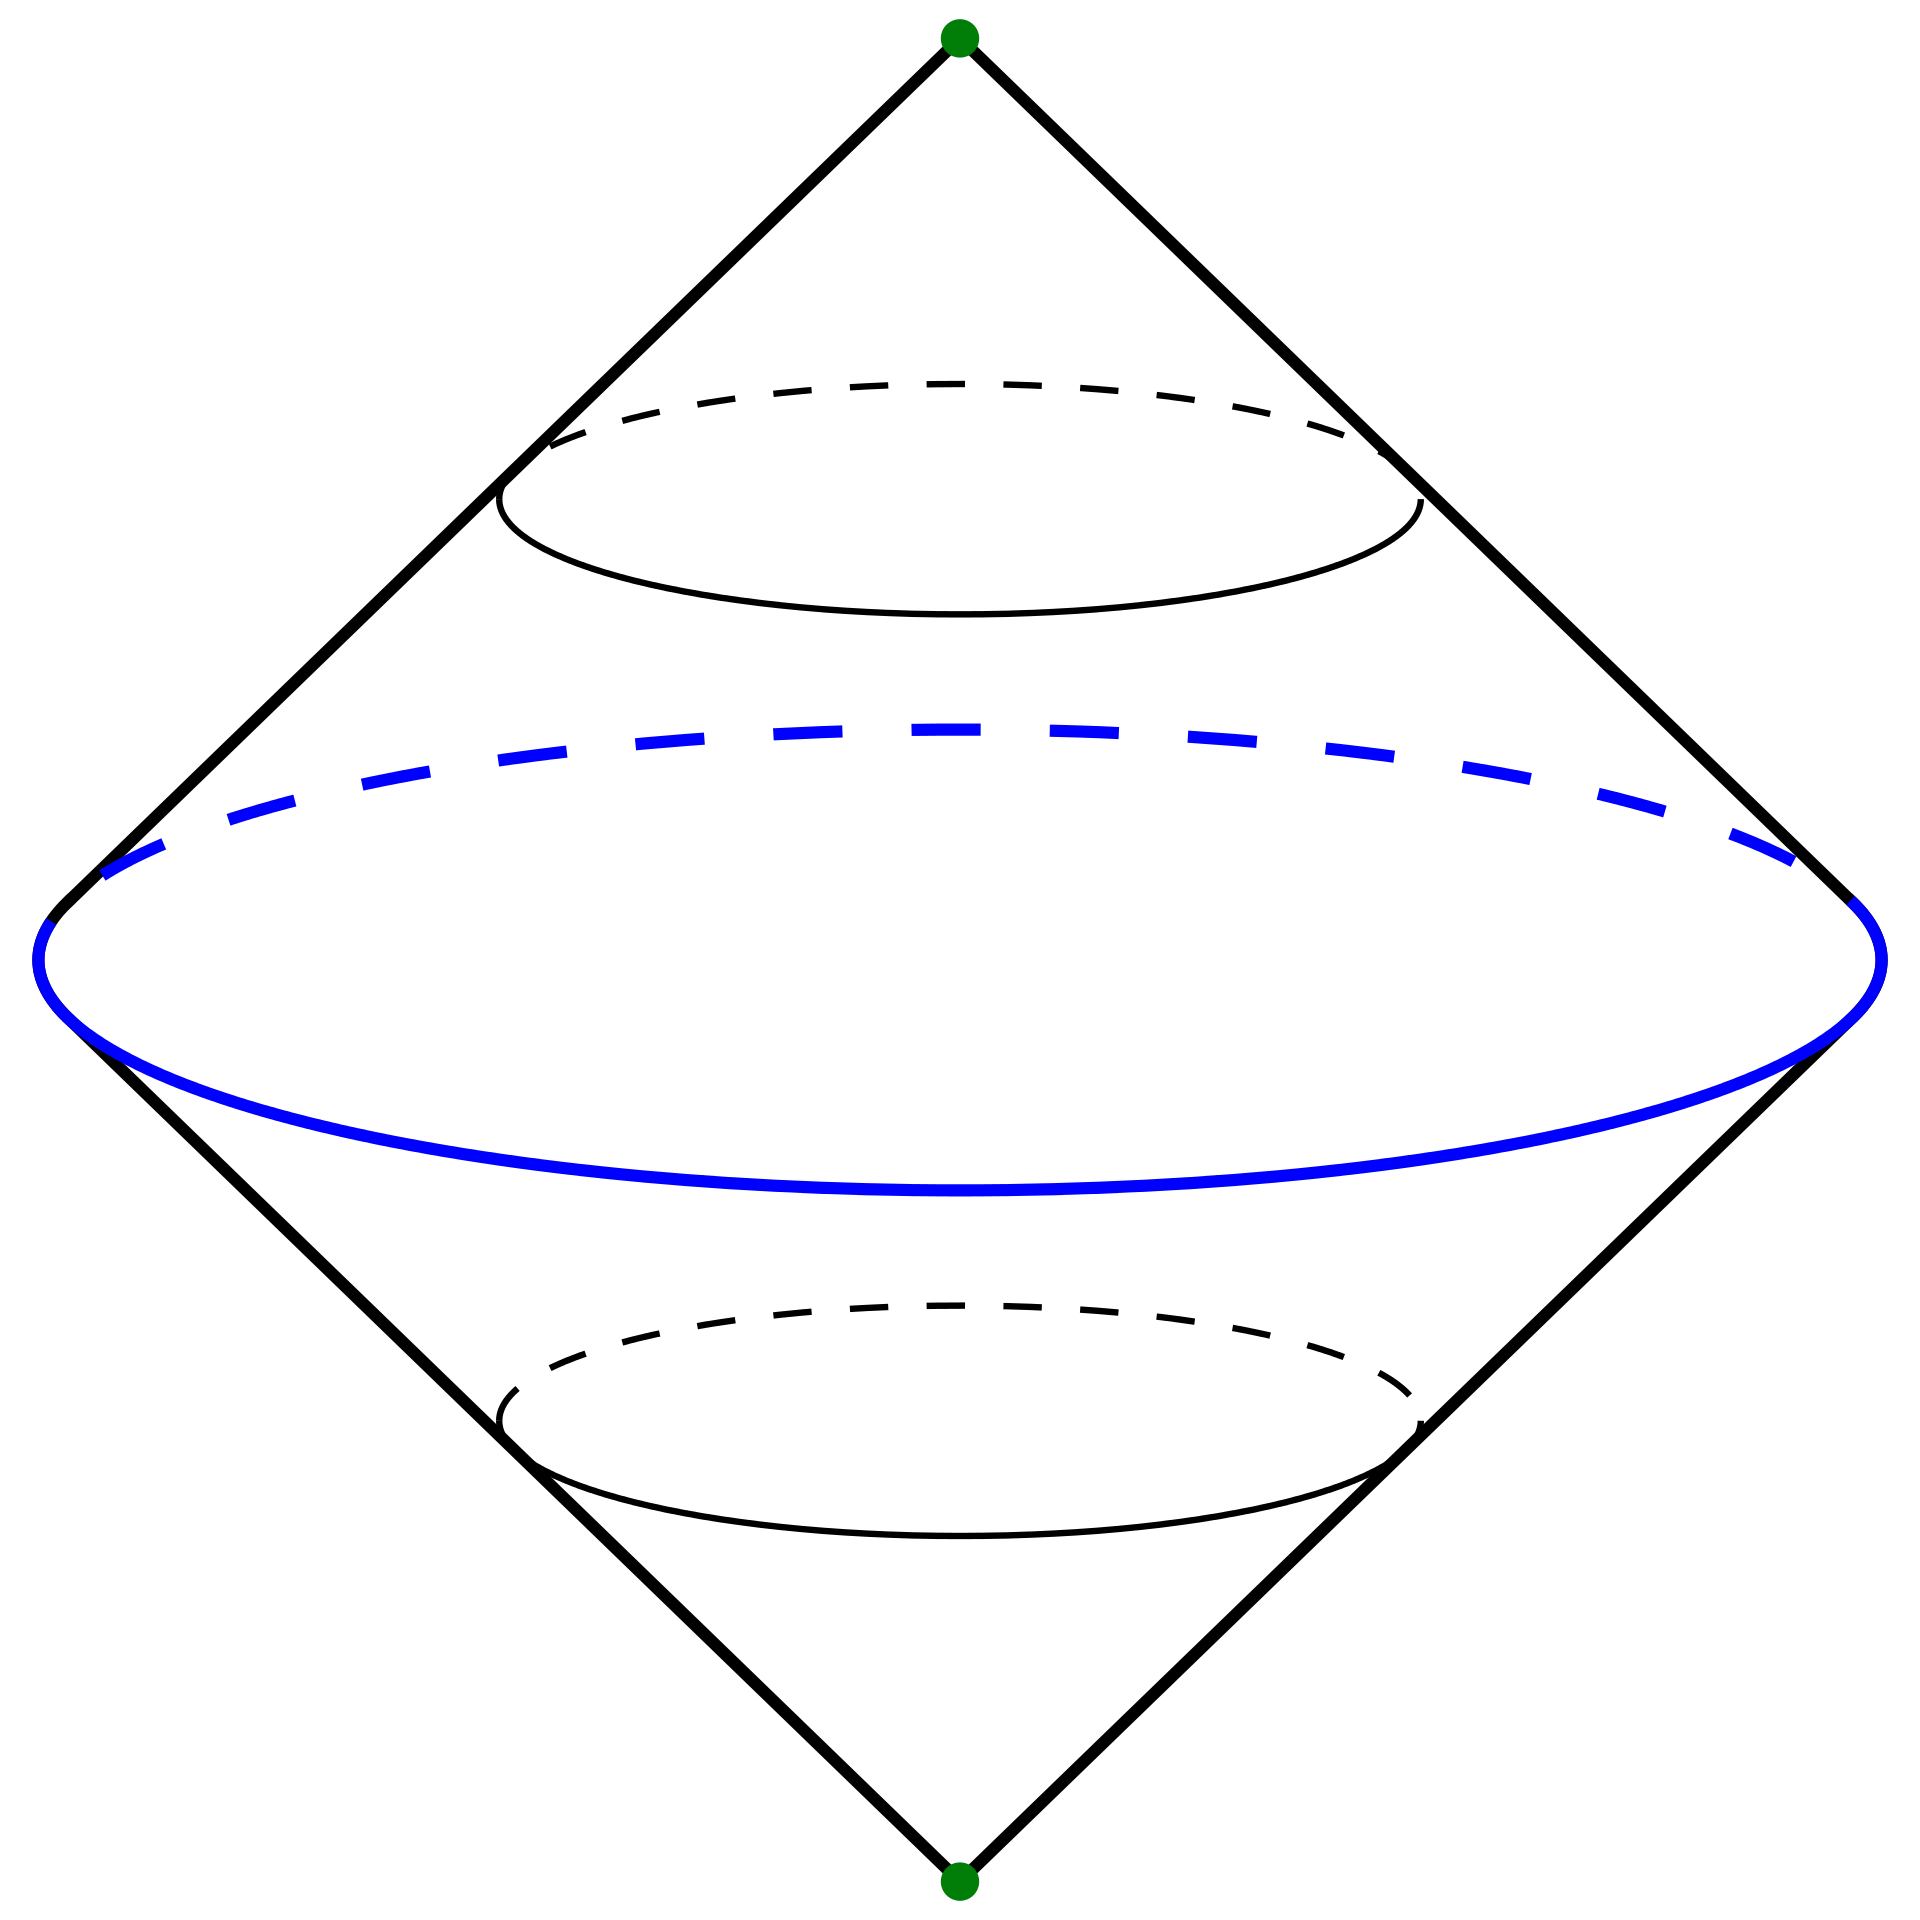
\includegraphics[scale = 0.05]{lectures/0/pictures/pic_5.svg}
        \end{center}
    \end{example}

    Так как надстройка получается факторизацией конуса по нижнему основанию, из теоремы о факторизации~\ref{FactorizationTheorem} следует, что $H_{q + 1}(CX, X) \cong \widetilde{H}_{q + 1}(\Sigma X)$.
    Таким образом, мы получили такое утверждение:
    \begin{theorem}[Гомологии надстройки]
        Справедливо следующее равенство групп гомологий:
        \[ \widetilde{H}_{q}(X) \cong \widetilde{H}_{q + 1}(\Sigma X) \]
    \end{theorem}

    \begin{remark}
       Так как $\Sigma S^n = S^{n + 1}$, мы таким образом получили другое доказательство теоремы~\ref{SphereHomology}.
    \end{remark}

    \begin{theorem}[Гомологии букета]\label{BouqetHomology}
        Для букета пространств $\bigvee_{\alpha} X_{\alpha}$ включения $i_{\alpha}\colon X_{\alpha} \hookrightarrow \bigvee_{\alpha} X_{\alpha}$
        индуцируют изоморфизм гомологий
        \[ \bigoplus_{\alpha} \widetilde{H}_{q} \cong \widetilde{H}_{q}\lr*{\bigvee_{\alpha} X_{\alpha}}. \]
        при условии, что если в букете отождествляются точки $\{ x_{\alpha} \}$, то пары $(X_{\alpha}, x_{\alpha})$~--- пары Борсука.
    \end{theorem}
    \begin{proof}
        Достаточно рассмотреть пару
        \[ (X, A) = \lr*{\bigsqcup_{\alpha} X_{\alpha}, \bigsqcup_{\alpha} x_{\alpha}}, \]
        тогда по тривиальным причинам
        \[ H_{n}(X, A) \cong \bigoplus_{\alpha} \widetilde{H}_{n}(X_{\alpha}) \]
        и по теореме о факторизации
        \[ H_{n}(X, A) \cong \widetilde{H}_{n}\lr*{\bigvee_{\alpha}X_{\alpha}}. \]
    \end{proof}

    \subsection{Гомологии с коэффициентами}

    У рассматриваемой нами до сих пор теории гомологий есть простое обобщение, котрое иногда даёт техническое преимущество.

    Обобщение состоит в рассмотрении цепей $\sum n_i f_i, $ где $f_i$~--- сингулярные симплексы, а коэффициенты $n_i$
    берутся в фиксированной абелевой группе $G$. Такие $n$-мерные цепи образуют абелеву группу $C_{n}(X; G)$ и у неё также есть относительная версия
    $C_{n}(X, A; G) \eqdef C_{n}(X; G)/ C_{n}(A; G)$.

    Дифференциал $\delta$ строится также, как и раньше:
    \[ \partial\lr*{\sum_{i} n_i f_i } = \sum_{i, j} (-1)^j n_i \Gamma_{j}f_i. \]
    Соотвественно, группы $C_{n}(X; G)$ и $C_{n}(X, A; G)$ образуют цепные комплексы и их гомологии обозначают
    $H_{n}(X; G)$ и $H_{n}(X, A; G)$ и называют \emph{гомологиями с коэффициентами в группе $G$}.

    Приведённые группы гомологий $\widetilde{H}(X; G)$ определяются аналогично, аугументация задаётся, как
    \[ \ldots \to C_{0}(X; G) \xrightarrow{\varepsilon} G \to 0, \quad \varepsilon\lr*{\sum_{i} n_i f_i} = \sum_{i} n_i.  \]

    \begin{remark}
       Часто полезно рассматривать гоиологии с коэффициентами в $\Z/2\Z$, так как нужно считать суммы сингулярных симплексов
        с коэффициентами $0$ и $1$, поэтому, отбрасывая члены с коэффициентами $0$, можно представлять себе цепи, как конечные <<объединения>> сингулярных симплексов.

        Кроме того, можно больше не заботиться о знаках в формуле для границы, а так как знаки являются алгебраическим выражением ориентации, мы можем игнорировать и ориентации.
        Это означает, что гомологии с коэффициентами в $\Z/2\Z$~--- наиболее естественный инструмент для вычислений в неориентируемом случае.
    \end{remark}

    Отметим, что вся доказанная выше теория переносится на гомологии с коэффициентами в $G$ без проблем и различия между
    $H_{n}(X; G)$ и $H_{n}(X)$ появляются только, когда начинаются вычисления.

    \begin{example}
        Если $X = *$~--- точка, то нетрудно заметить, что
        \[ H_{n}(*; G) \cong \begin{cases} G, \quad n = 0 \\ 0, \quad \text{иначе} \end{cases}\]

        Аналогично и в случае сфер $S^k$ мы имеем
        \[ \widetilde{H}_{n}(S^k; G) \cong \begin{cases} G, \quad n = k \\ 0, \quad \text{иначе} \end{cases}\]
    \end{example}










